\section{Robust Regression}

\subsection{Recommended References}
\begin{frame}{Recommended References}
	\begin{vfilleditems}
		\item \textcite{gelman2013bayesian} - Chapter 17: Models for robust inference
		\item \textcite{mcelreath2020statistical} - Chapter 12: Monsters and Mixtures
		\item \textcite{gelman2020regression}:
		\begin{vfilleditems}
			\item Chapter 15, Section 15.6: Robust regression using the t model
			\item Chapter 15, Section 15.8: Going beyond generalized linear models
		\end{vfilleditems}
	\end{vfilleditems}
\end{frame}

\begin{frame}{Robust Models\footnote{\href{https://github.com/allisonhorst/stats-illustrations}{figure from Allison Horst (CC-BY-4.0)}.}}
	\begin{columns}
		\begin{column}{0.6\textwidth}
			Almost always data from real world are really strange.
			\vfill
			For the sake of convenience, we use simple models.
			But always ask yourself.
			How many ways might the posterior inference depends on the following:
			\vfill
			\begin{vfilleditems}
				\item extreme observations (outliers)?
				\item unrealistic model assumptions?
			\end{vfilleditems}
		\end{column}
		\begin{column}{0.4\textwidth}
			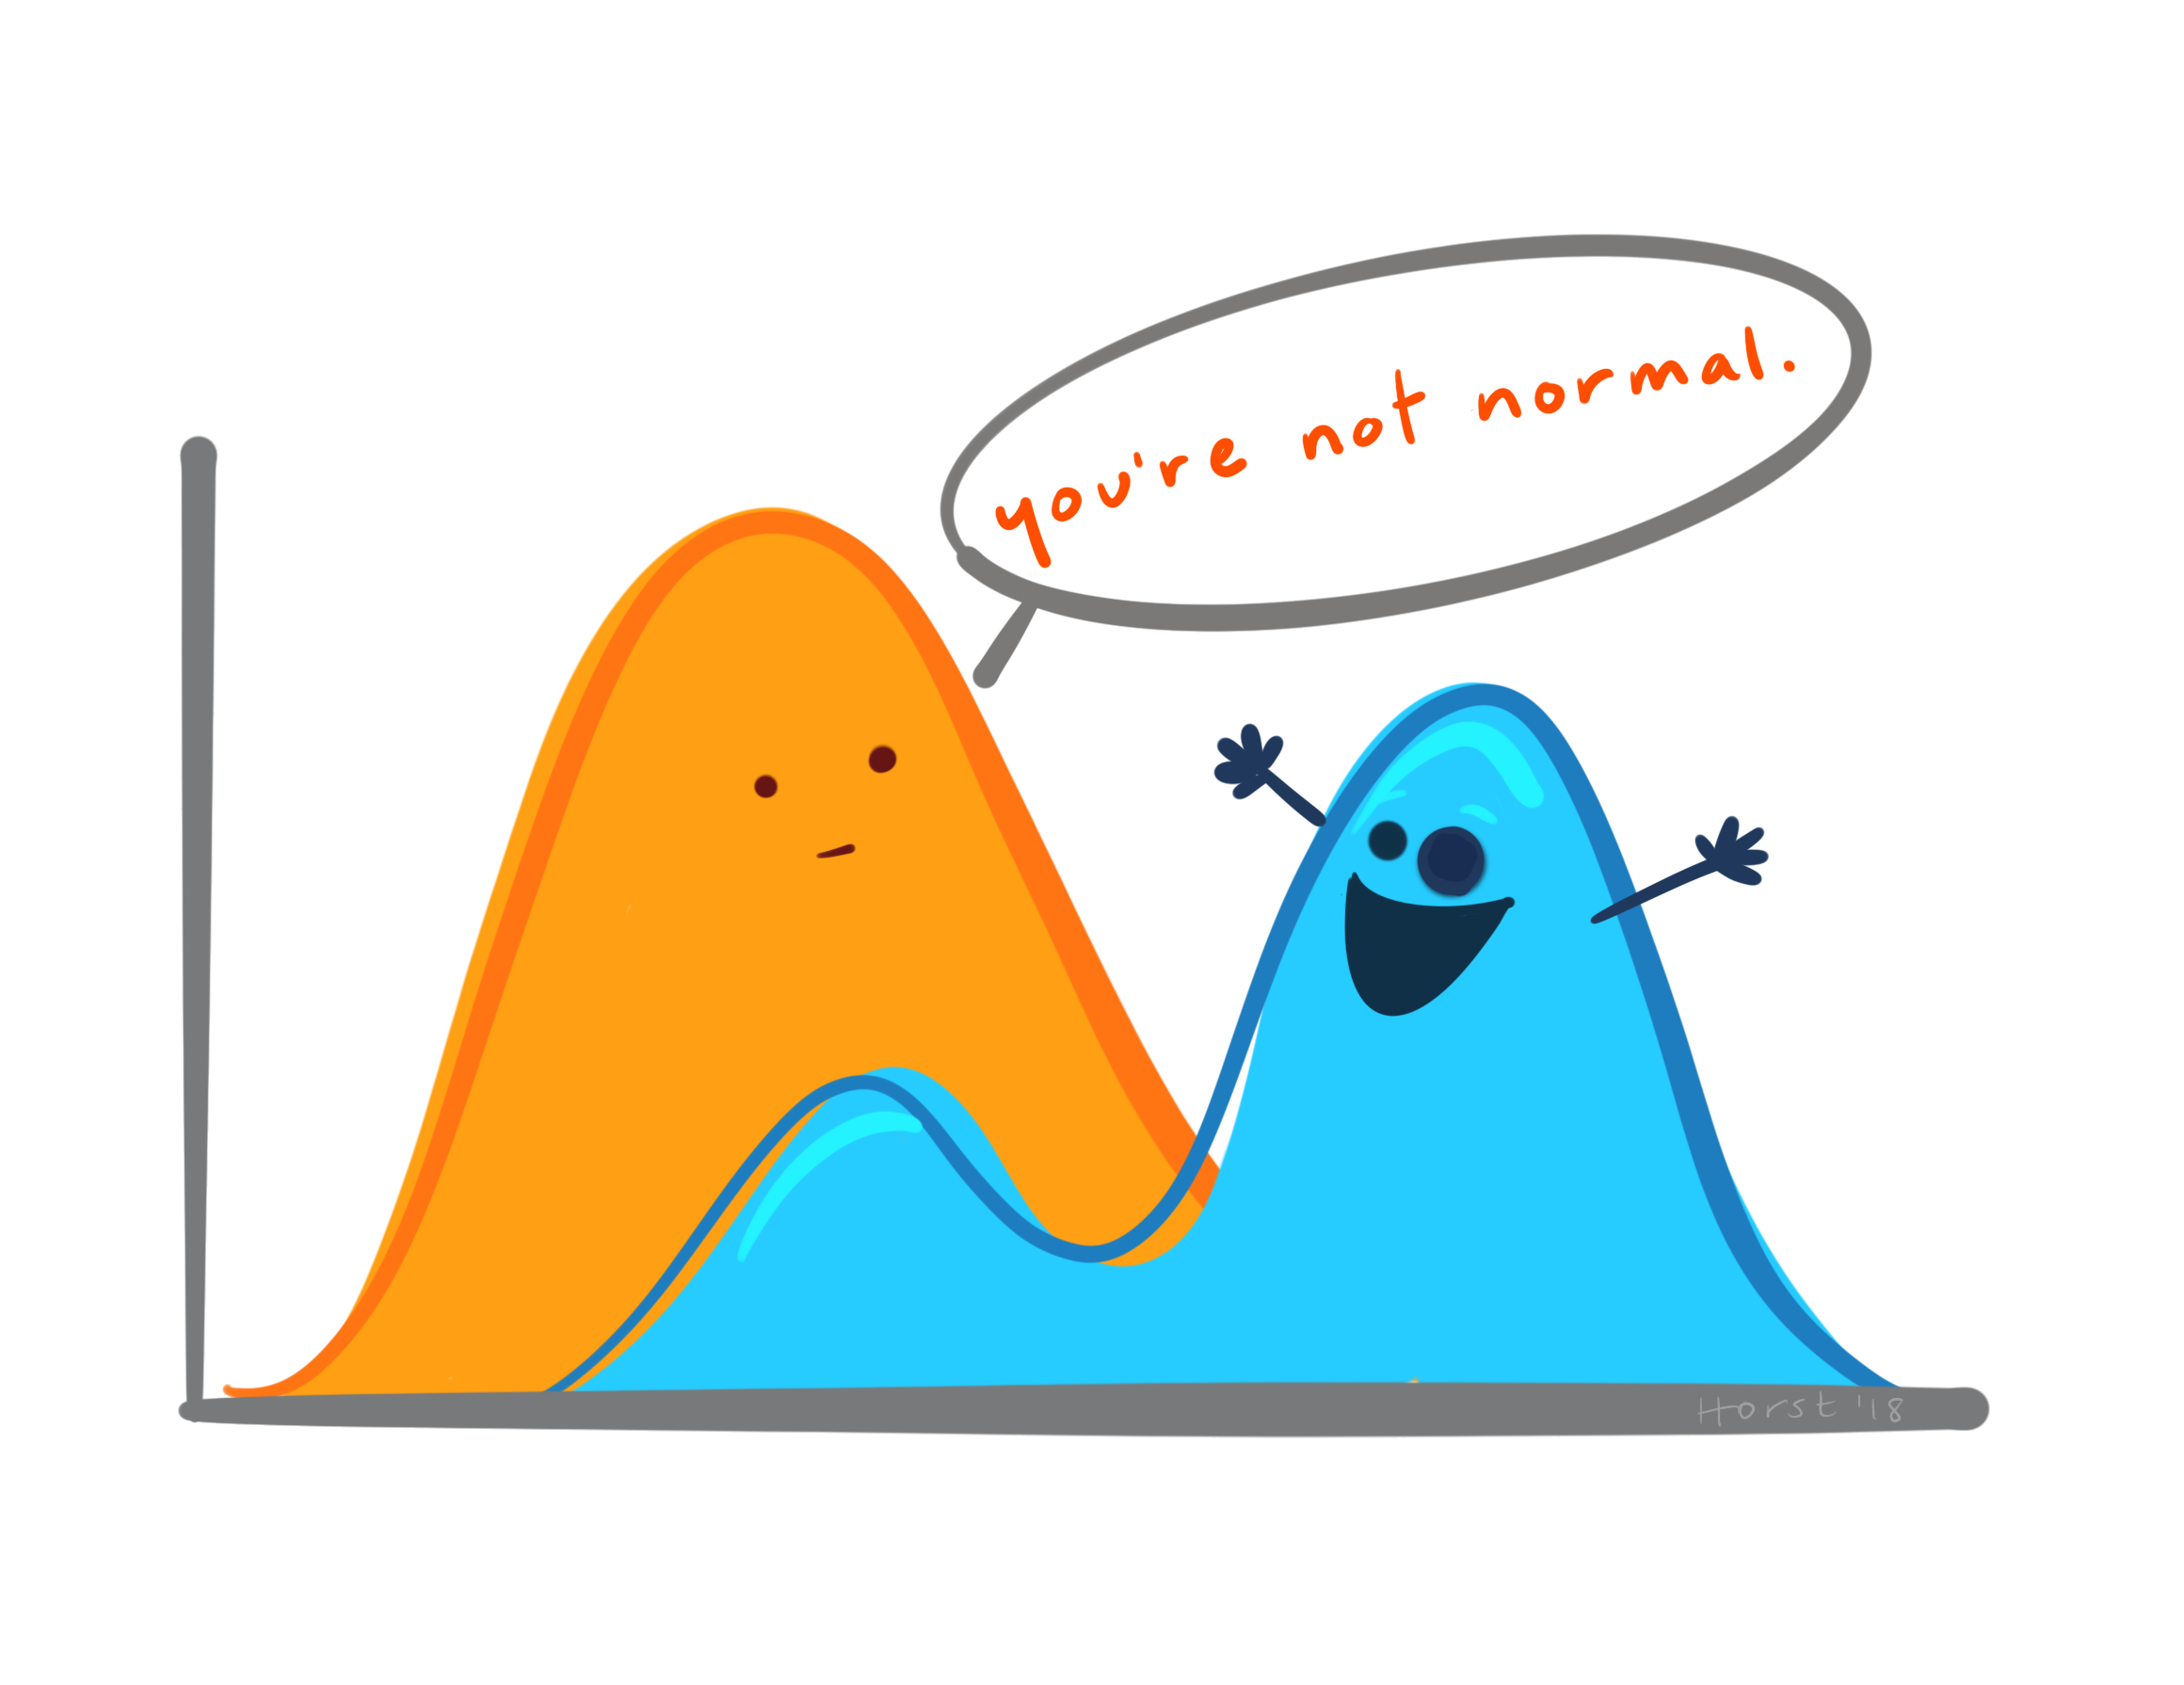
\includegraphics[width=0.9\columnwidth]{not_normal_transparent.png}
		\end{column}
	\end{columns}
\end{frame}

\subsection{Outliers}
\begin{frame}{Outliers}
	Models based on the \textbf{normal distribution are notoriously ``non-robust''
		against outliers},
	in the sense that a \textbf{single observation can greatly affect the
		inference of all model's parameters},
	even those that has a shallow relationship with it.
\end{frame}

\subsection{Overdispersion}
\begin{frame}{Overdispersion}
	\begin{defn}[Overdispersion and underdispersion]
		Superdispersion and underdispersion\footnote{
			rarer to find in the real world.}
		refer to data that have more or fewer variation than expected
		under a probability model.
		\parencite{gelman2020regression}
	\end{defn}
	\vfill
	For each one of the models we covered, there is a \textbf{natural extension}
	in which \textbf{a single parameter} is added to allow for overdispersion.
	\parencite{gelman2013bayesian}.
\end{frame}

\begin{frame}{Overdispersion Example}
	\begin{example}[Car accidents]
		Suppose you are analyzing data from car accidents.
		The model we generally use in this type of phenomena is
		\textbf{Poisson regression}.
		\vfill
		Poisson distribution has the same parameter for both the mean and variance:
		the rate parameter $\lambda$.
		\vfill
		Hence, if you find a higher variability than expected under the
		Poisson likelihood function allows,
		then probably you won't be able to model properly the desired phenomena.
	\end{example}
\end{frame}

\subsection{Overdispersion Versions of Probabilistic Models}
\subsubsection{Student's $t$ instead of Normal}
\begin{frame}{Student's $t$ instead of Normal}
	Student's $t$ distribution has \textbf{wider\footnote{or ``fatter''.} tails}
	than the Normal distribution.
	\vfill
	This makes it a good candidate to \textbf{fit outliers without
		instabilities in the parameters' inference}.
	\vfill
	From the Bayesian viewpoint, there is nothing special or magical in the
	Gaussian/Normal likelihood.
	It is just another distribution specified in a statistical model.
	We can make our model robust by using the Student's $t$ distribution
	as a likelihood function.
\end{frame}

\begin{frame}{Student's $t$ instead of Normal}
	\centering
	\begin{tikzpicture}
		\begin{axis}[every axis plot, line width=2pt,
				ylabel=PDF,
				domain=-4:4,samples=200,
				axis x line*=bottom, % no box around the plot, only x and y axis
				axis y line*=left % the * suppresses the arrow tips
			]

			\addplot [blue] {gaussian(0, 1)};
			\addlegendentry{Normal}
			\addplot [red] {student(3)};
			\addlegendentry{Student's $t$ with $\nu=3$}
		\end{axis}
	\end{tikzpicture}
\end{frame}

\begin{frame}{Student's $t$ instead of Normal}
	By using a Student's $t$ distribution instead of the Normal distribution
	as likelihood functions,
	the model's error $\sigma$ does \textit{not} follow a Normal distribution,
	but a Student's $t$ distribution:
	$$
		\begin{aligned}
			\boldsymbol{y}     & \sim \text{Student}\left( \nu, \alpha + \mathbf{X} \boldsymbol{\beta}, \sigma \right) \\
			\alpha             & \sim \text{Normal}(\mu_\alpha, \sigma_\alpha)                                         \\
			\boldsymbol{\beta} & \sim \text{Normal}(\mu_{\boldsymbol{\beta}}, \sigma_{\boldsymbol{\beta}})             \\
			\nu                & \sim \text{Log-Normal}(2, 1)                                                          \\
			\sigma             & \sim \text{Exponential}(\lambda_\sigma)
		\end{aligned}
	$$
	\small
	Note that we are including an extra parameter $\nu$,
	which representes the Student's $t$ distribution degrees of freedom,
	to be estimated by the model \parencite{gelman2013bayesian}.
	This controls how wide or narrow the ``tails'' of the distribution will be.
	A heavy-tailed, positive-only prior is advised.
\end{frame}

\subsubsection{Beta-Binomial instead of Binomial}
\begin{frame}{Beta-Binomial instead of the Binomial}
	The binomial distribution has a practical limitation that we only have
	one free parameter to estimate\footnote{since $n$ already comes from data.} ($p$).
	This implies in the \textbf{variance to determined by the mean}.
	Hence, the binomial distribution \textbf{cannot} tolerate overdispersion.
	\vfill
	A robust alternative is the \textbf{beta-binomial distribution}, which,
	as the name suggests, is a \textbf{beta mixture of binomials distributions}.
	Most important, it \textbf{allows that the variance to be independent of the mean},
	making it \textbf{robust against overdispersion}.
\end{frame}

\begin{frame}{Beta-Binomial instead of Binomial}
	The \textbf{beta-binomial distribution} is a binomial distribution, where
	the probability of success $p$ is parameterized as a $\text{Beta}(\alpha, \beta)$.
	\vfill
	Generally, we use $\alpha$ as the binomial's probability of the success $p$,
	and $\beta$\footnote(sometimes specified as $\phi$) is the additional parameter
	to control and allow for overdispersion.
	\vfill
	Values of $\beta \geq 1$ make the beta-binomial behave the same as a binomial.
\end{frame}

\begin{frame}{Beta-Binomial instead of Binomial}
	$$
		\begin{aligned}
			\boldsymbol{y}     & \sim \text{Beta-Binomial}(n, p, \phi)                                     \\
			p                  & \sim \text{Logistic/Probit}(\alpha +  \mathbf{X} \boldsymbol{\beta})     \\
			\alpha             & \sim \text{Normal}(\mu_\alpha, \sigma_\alpha)                             \\
			\boldsymbol{\beta} & \sim \text{Normal}(\mu_{\boldsymbol{\beta}}, \sigma_{\boldsymbol{\beta}}) \\
			\phi               & \sim \text{Exponential}(1)
		\end{aligned}
	$$
	\vfill
	It is also proper to include the overdispersion $\beta$ parameter as an
	additional parameter to be estimated by the model
	\parencite{gelman2013bayesian,mcelreath2020statistical}.
	A heavy-tailed, positive-only prior is advised.
\end{frame}

\subsubsection{Student's $t$ instead Binomial}
\begin{frame}{Student's $t$ instead Binomial}
	\small
	Also known as Robit\footnote{there is a great discussion between
		Gelman, Vehtari and Kurz at
		\href{https://discourse.mc-stan.org/t/robit-regression-not-robust/21245/}{
			\texttt{Stan}'s Discourse}.} \parencite{gelman2013bayesian, gelman2020regression}.
	The ideia is to make the logistic regression robust by using a
	\textbf{latent variable $z$} as the linear predictor.
	$z$'s errors, $\epsilon$, are distributed as a Student's $t$ distribution:
	$$
		\begin{aligned}
			y_i        & = \begin{cases} 0 & \text{se } z_i < 0 \\ 1 & \text{se }\ z_i > 0 \end{cases} \\
			z_i        & = X_i \boldsymbol{\beta} + \epsilon_i                                         \\
			\epsilon_i & \sim \text{Student} \left (\nu, 0, \sqrt{\frac{\nu - 2}{\nu}} \right)         \\
			\nu        & \sim \text{Gamma}(2, 0.1) \in \left[2, \infty \right)
		\end{aligned}
	$$
	\footnotesize
	Here we are using the gamma distribution as a truncated Student's $t$
	distribution for the degrees of freedom parameter $\nu \geq 2$.
	Another option would be to fix $\nu = 4$.
\end{frame}

\subsubsection{Negative Binomial instead of Poisson}
\begin{frame}{Negative Binomial instead of Poisson}
	This is the overdispersion example.
	The Poisson distribution uses a \textbf{single parameter for both its mean and variance}.
	\vfill
	Hence, if you find overdispersion, probably you'll need a robust alternative to Poisson.
	This is where the \textbf{negative binomial}, with an extra parameter $\phi$,
	that makes it \textbf{robust to overdispersion}.
	\vfill
	$\phi$ controls the probability of success $p$,
	and we generally use a gamma distribution as its prior.
	$\phi$ is also known as a ``reciprocal dispersion'' parameter.
\end{frame}

\begin{frame}{Negative Binomial instead of Poisson}
	$$
		\begin{aligned}
			\boldsymbol{y}     & \sim \text{Negative Binomial} \left( e^{(\alpha + \mathbf{X} \boldsymbol{\beta})}, \phi \right) \\
			\phi               & \sim \text{Gamma}(0.01, 0.01)                                                                   \\
			\alpha             & \sim \text{Normal}(\mu_\alpha, \sigma_\alpha)                                                   \\
			\boldsymbol{\beta} & \sim \text{Normal}(\mu_{\boldsymbol{\beta}}, \sigma_{\boldsymbol{\beta}})
		\end{aligned}
	$$
	\vfill
	Here we also give a heavy-tailed, positive-only prior to $\phi$.
	Something like the $\text{Gamma}(0.01, 0.01)$ works.
\end{frame}

\subsubsection{Negative Binomial Mixture instead of Poisson}
\begin{frame}{Negative Binomial Mixture instead of Poisson}
	Even using a negative binomial likelihood,
	if you encounter acute overdispersion,
	specially when there is a lot of zeros in your data
	(zero-inflated),
	your model can still perform a bad fit to the data.
	\vfill
	Another suggestion is to use a mixture of negative binomial
	\parencite{mcelreath2020statistical}.
\end{frame}

\begin{frame}{Negative Binomial Mixture instead of Poisson}
	Here, $S_i$ is a dummy variable,
	taking value $1$ if the $i$th observation has a value $\neq 0$.
	$S_i$ can be modeled using logistic regression:
	$$
		\begin{aligned}
			\boldsymbol{y}
			                    & \begin{cases}
				                      = 0,                                                                                             & \text{ if } S_i = 0 \\
				                      \sim \text{Negative Binomial} \left( e^{(\alpha + \mathbf{X} \boldsymbol{\beta})}, \phi \right), & \text{ if } S_i = 1
			                      \end{cases} \\
			P(S_i = 1)          & = \text{Logistic/Logit}(\mathbf{X} \boldsymbol{\gamma})                                                               \\
			\boldsymbol{\gamma} & \sim \text{Beta}(1, 1)
		\end{aligned}
	$$
	\vfill
	$\boldsymbol{\gamma}$ is a new vector of coefficients which we give uniform priors of $\text{Beta} (1, 1)$.
\end{frame}

\subsection{Why Use Non-Robust Models?}
\begin{frame}{Why Use Non-Robust Models?}
	The \textbf{central limit theorem} tells us that the \textbf{normal distribution}
	is an appropriate model for data that arises as a
	\textbf{sum of independent components}.
	\vfill
	Even when they are naturally not implicit in a phenomena structure,
	\textbf{simpler non-robust models are computational efficient}.
	\vfill
	Of course, you must always guide the model choice in a
	\textbf{principled manner},
	taking into account the underlying phenomena data generating process.
	And make sure to make \textbf{posterior predictive checks}.
\end{frame}
